\section*{Control}
\subsection*{PD controller with gravity compensation}
    The first controller that is going to be tested is a simple PD controller with gravity compensation:
    $$
        u=K_p\tilde{q} - K_d\dot{q} +g(q)
    $$
     where $\tilde{q} = q_d - q$ and 
     \begin{align}\label{eq:gravity}
     g(q) = \frac{\partial P}{\partial q_k}
     \end{align}

     
     and the total potential energy for a n-link robot is $P = \sum^n_{i=1}P_i$. Where $P_i$ is the potential energy for each individual link. For this specific manipulator the center of mass is assumed in the geometric center of each link. 
     \\
     Using figure \figref{draw:pot-rob} to calculate the potential energies:

     
     \begin{align*}
        P_1 &= 0
        \\
        P_2 &= m_2g\frac{L_2}{2}\sin{(q_2)}
        \\
        P_3 &= m_3g\left( L_2 \sin{(q_2)} + \frac{L_3}{2}\sin{(q_2 + q_3)} \right)
        \\
        P_4 &= m_4g\left( L_2 \sin{(q_2)} + L_3\sin{(q_2 + q_3)} + \frac{L_4}{2}\sin{(q_2+q_3+q_4)} \right)
        \\
        P_5 &= m_5g\left( L_2 \sin{(q_2)} + L_3\sin{(q_2 + q_3)} + \left(L_4 + \frac{L_5}{2} \right)\sin{(q_2+q_3+q_4)} \right)
        \\
        P &= P_1 + P_2 + P_3 + P_4 + P_5
     \end{align*}

     $L_4$ is the part up to the rotational joint. $L_5$ and $m_5$ is the rotational joint and the gripper together. To calculate individual gravity components we are using \eqref{eq:gravity}

     \begin{align*}
        g_1 &= 0
        \\
        g_2 &= \frac{\partial P}{\partial q_2} = 
        m_2g\frac{L_2}{2}\cos{(q_2)}+
        m_3g\left( L_2 \cos{(q_2)} + \frac{L_3}{2}\cos{(q_2+q_3)} \right)\\&+
        m_4g\left( L_2 \cos{(q_2)} + L_3\cos{(q_2 + q_3)} + \frac{L_4}{2}\cos{(q_2+q_3+q_4)} \right)\\&+
        m_5g\left( L_2 \cos{(q_2)} + L_3\cos{(q_2 + q_3)} + \left(L_4 + \frac{L_5}{2} \right)\cos{(q_2+q_3+q_4)} \right)
        \\
        g_3 &= \frac{\partial P}{\partial q_3} =
        m_3g\frac{L_3}{2}\cos{(q_2+q_3)} +
        m_4g\left( L_3\cos{(q_2 + q_3)} + \frac{L_4}{2}\cos{(q_2+q_3+q_4)} \right)\\&+
        m_5g\left(  L_3\cos{(q_2 + q_3)} + \left(L_4 + \frac{L_5}{2} \right)\cos{(q_2+q_3+q_4)} \right)
        \\
        g_4 &=\frac{\partial P}{\partial q_4} = 
        m_4g\frac{L_4}{2}\cos{(q_2+q_3+q_4)}+
        m_5g\left(L_4 + \frac{L_5}{2} \right)\cos{(q_2+q_3+q_4)}
        \\
        g_5 &= 0
        \\
        g(q) &= [g_1,g_2,g_3,g_4,g_5]^T
     \end{align*}

NOTE to self: Since the manipulator zero position is straight upwards this calculation is wrong. Replace sin with cos and vice versa. Remember signs. 

\begin{figure}[htbp]
    \centering
    

%Thank you http://www.texample.net/tikz/examples/three-link-annotated/

\usetikzlibrary{patterns}

\newcommand{\nvar}[2]{%
    \newlength{#1}
    \setlength{#1}{#2}
}

% Define a few constants for drawing
\nvar{\dg}{0.3cm}
\def\dw{0.25}\def\dh{0.5}
\nvar{\ddx}{1.5cm}

% Define commands for links, joints and such
\def\link{\draw [double distance=1.5mm, very thick] (0,0)--}
\def\joint{%
    \filldraw [fill=white] (0,0) circle (5pt);
    \fill[black] circle (2pt);
}
\def\grip{%
    \draw[ultra thick](0cm,\dg)--(0cm,-\dg);
    \fill (0cm, 0.5\dg)+(0cm,1.5pt) -- +(0.6\dg,0cm) -- +(0pt,-1.5pt);
    \fill (0cm, -0.5\dg)+(0cm,1.5pt) -- +(0.6\dg,0cm) -- +(0pt,-1.5pt);
}
\def\robotbase{%
    \draw[rounded corners=8pt] (-\dw,-\dh)-- (-\dw, 0) --
        (0,\dh)--(\dw,0)--(\dw,-\dh);
    \draw (-0.5,-\dh)-- (0.5,-\dh);
    \fill[pattern=north east lines] (-0.5,-1) rectangle (0.5,-\dh);
}

% Draw an angle annotation
% Input:
%   #1 Angle
%   #2 Label
% Example:
%   \angann{30}{$\theta_1$}
\newcommand{\angann}[2]{%
    \begin{scope}[red]
    \draw [dashed, red] (0,0) -- (0pt,1.2\ddx);
    \draw [dashed, red] (0,0) -- (1.2\ddx,0pt);
    \draw [->, shorten >=3.5pt] ((0,\ddx) arc (90:#1:\ddx);
    % Unfortunately automatic node placement on an arc is not supported yet.
    % We therefore have to compute an appropriate coordinate ourselves.
    \node at (#1*2+2:\ddx-8pt) {#2};
    \end{scope}
}

% Draw line annotation
% Input:
%   #1 Line offset (optional)
%   #2 Line angle
%   #3 Line length
%   #5 Line label
% Example:
%   \lineann[1]{30}{2}{$L_1$}
\newcommand{\lineann}[4][0.5]{%
    \begin{scope}[rotate=#2, blue,inner sep=2pt]
        \draw[dashed, blue!40] (0,0) -- +(0,#1)
            node [coordinate, near end] (a) {};
        \draw[dashed, blue!40] (#3,0) -- +(0,#1)
            node [coordinate, near end] (b) {};
        \draw[|<->|] (a) -- node[fill=white] {#4} (b);
    \end{scope}
}

% Define the kinematic parameters of the three link manipulator.
\def\thetaone{30}
\def\Lone{2}
\def\thetatwo{30}
\def\Ltwo{1}
\def\thetathree{40}
\def\Lthree{1}


\begin{tikzpicture}
    %\robotbase
    \angann{\thetaone}{$q_2$}
    \lineann[-1]{\thetaone}{\Lone}{$L_2$}
    \link(\thetaone:\Lone);
    \joint
    \begin{scope}[shift=(\thetaone:\Lone), rotate=\thetaone]
        \angann{\thetatwo}{$q_3$}
        \lineann[-1.5]{\thetatwo}{\Ltwo}{$L_3$}
        \link(\thetatwo:\Ltwo);
        \joint
        \begin{scope}[shift=(\thetatwo:\Ltwo), rotate=\thetatwo]
            \angann{\thetathree}{$q_4$}
            \lineann[-1]{\thetathree}{\Lthree}{$L_4$}
            \draw [dashed, red,rotate=\thetathree] (0,0) -- (1.2\ddx,0pt);
            \link(\thetathree:\Lthree);
            \joint
            \begin{scope}[shift=(\thetathree:\Lthree), rotate=\thetathree]
                %\grip
            \end{scope}
        \end{scope}
    \end{scope}
\end{tikzpicture}

    \caption{Figure of the robot. The twisting joints are left out}
    \label{draw:pot-rob}
\end{figure}


\subsection*{Tests with step response.}
In \figref{fig:testkp1} and \figref{fig:testkp2} the step response for the joint angles are plotted. \figref{fig:testkp1} is the joint angles when $kp = 1$ for the rotational joints ($q_2$ to $q_4$) and $kp = 1.5$ for the twist joints.  \figref{fig:testkp2} is the joint angles when $kp = 2$ for the rotational joints and $kp = 1.5$ for the twist joints. From the plots one can see that with a $kp$ bigger than $2$ will lead to unwanted oscillations. $kp = 1$ looks like the best choice for this controller so far. Keep in mind that this is the step response. The next step will be to make a spline to such that the steps are not so big. $kd = 0.9$ for the rotational joints bigger than this will cause weird oscillations.

\begin{figure}[htbp]
  \centering
  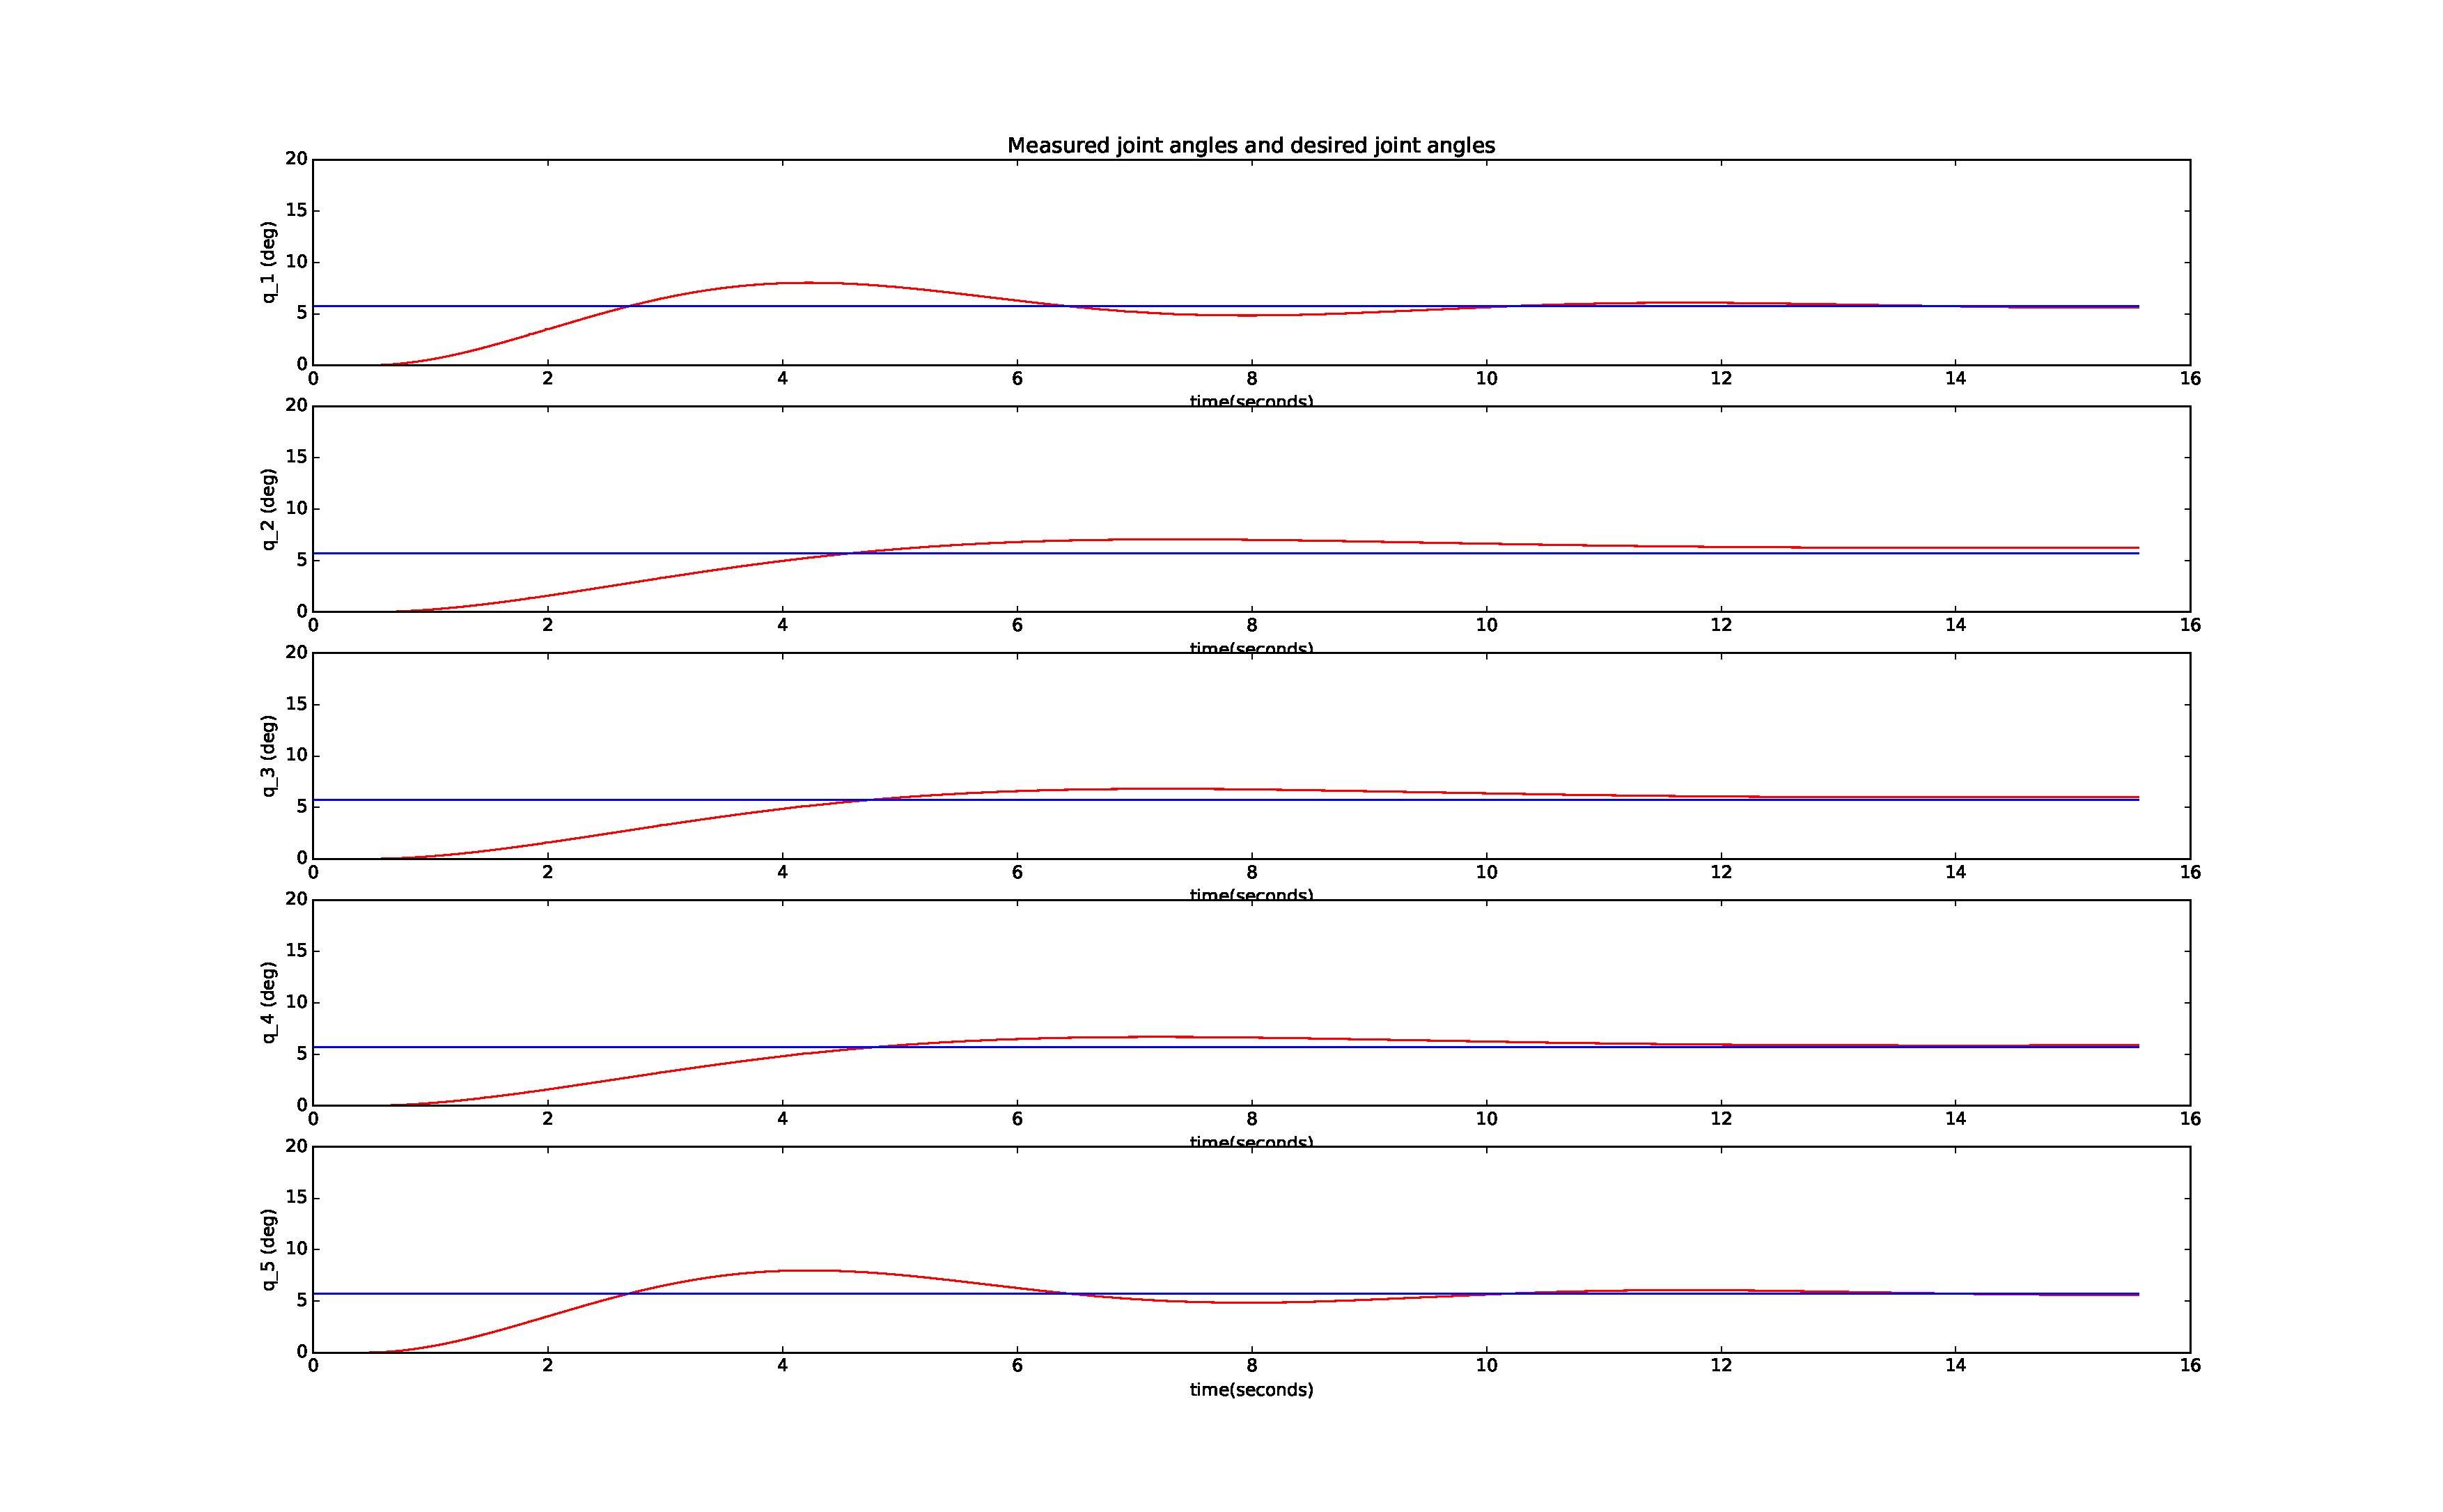
\includegraphics[width=.9\textwidth]{img/joingangKp1.eps}
  \caption{}
  \label{fig:testkp1}
\end{figure}
\begin{figure}[htbp]
  \centering
  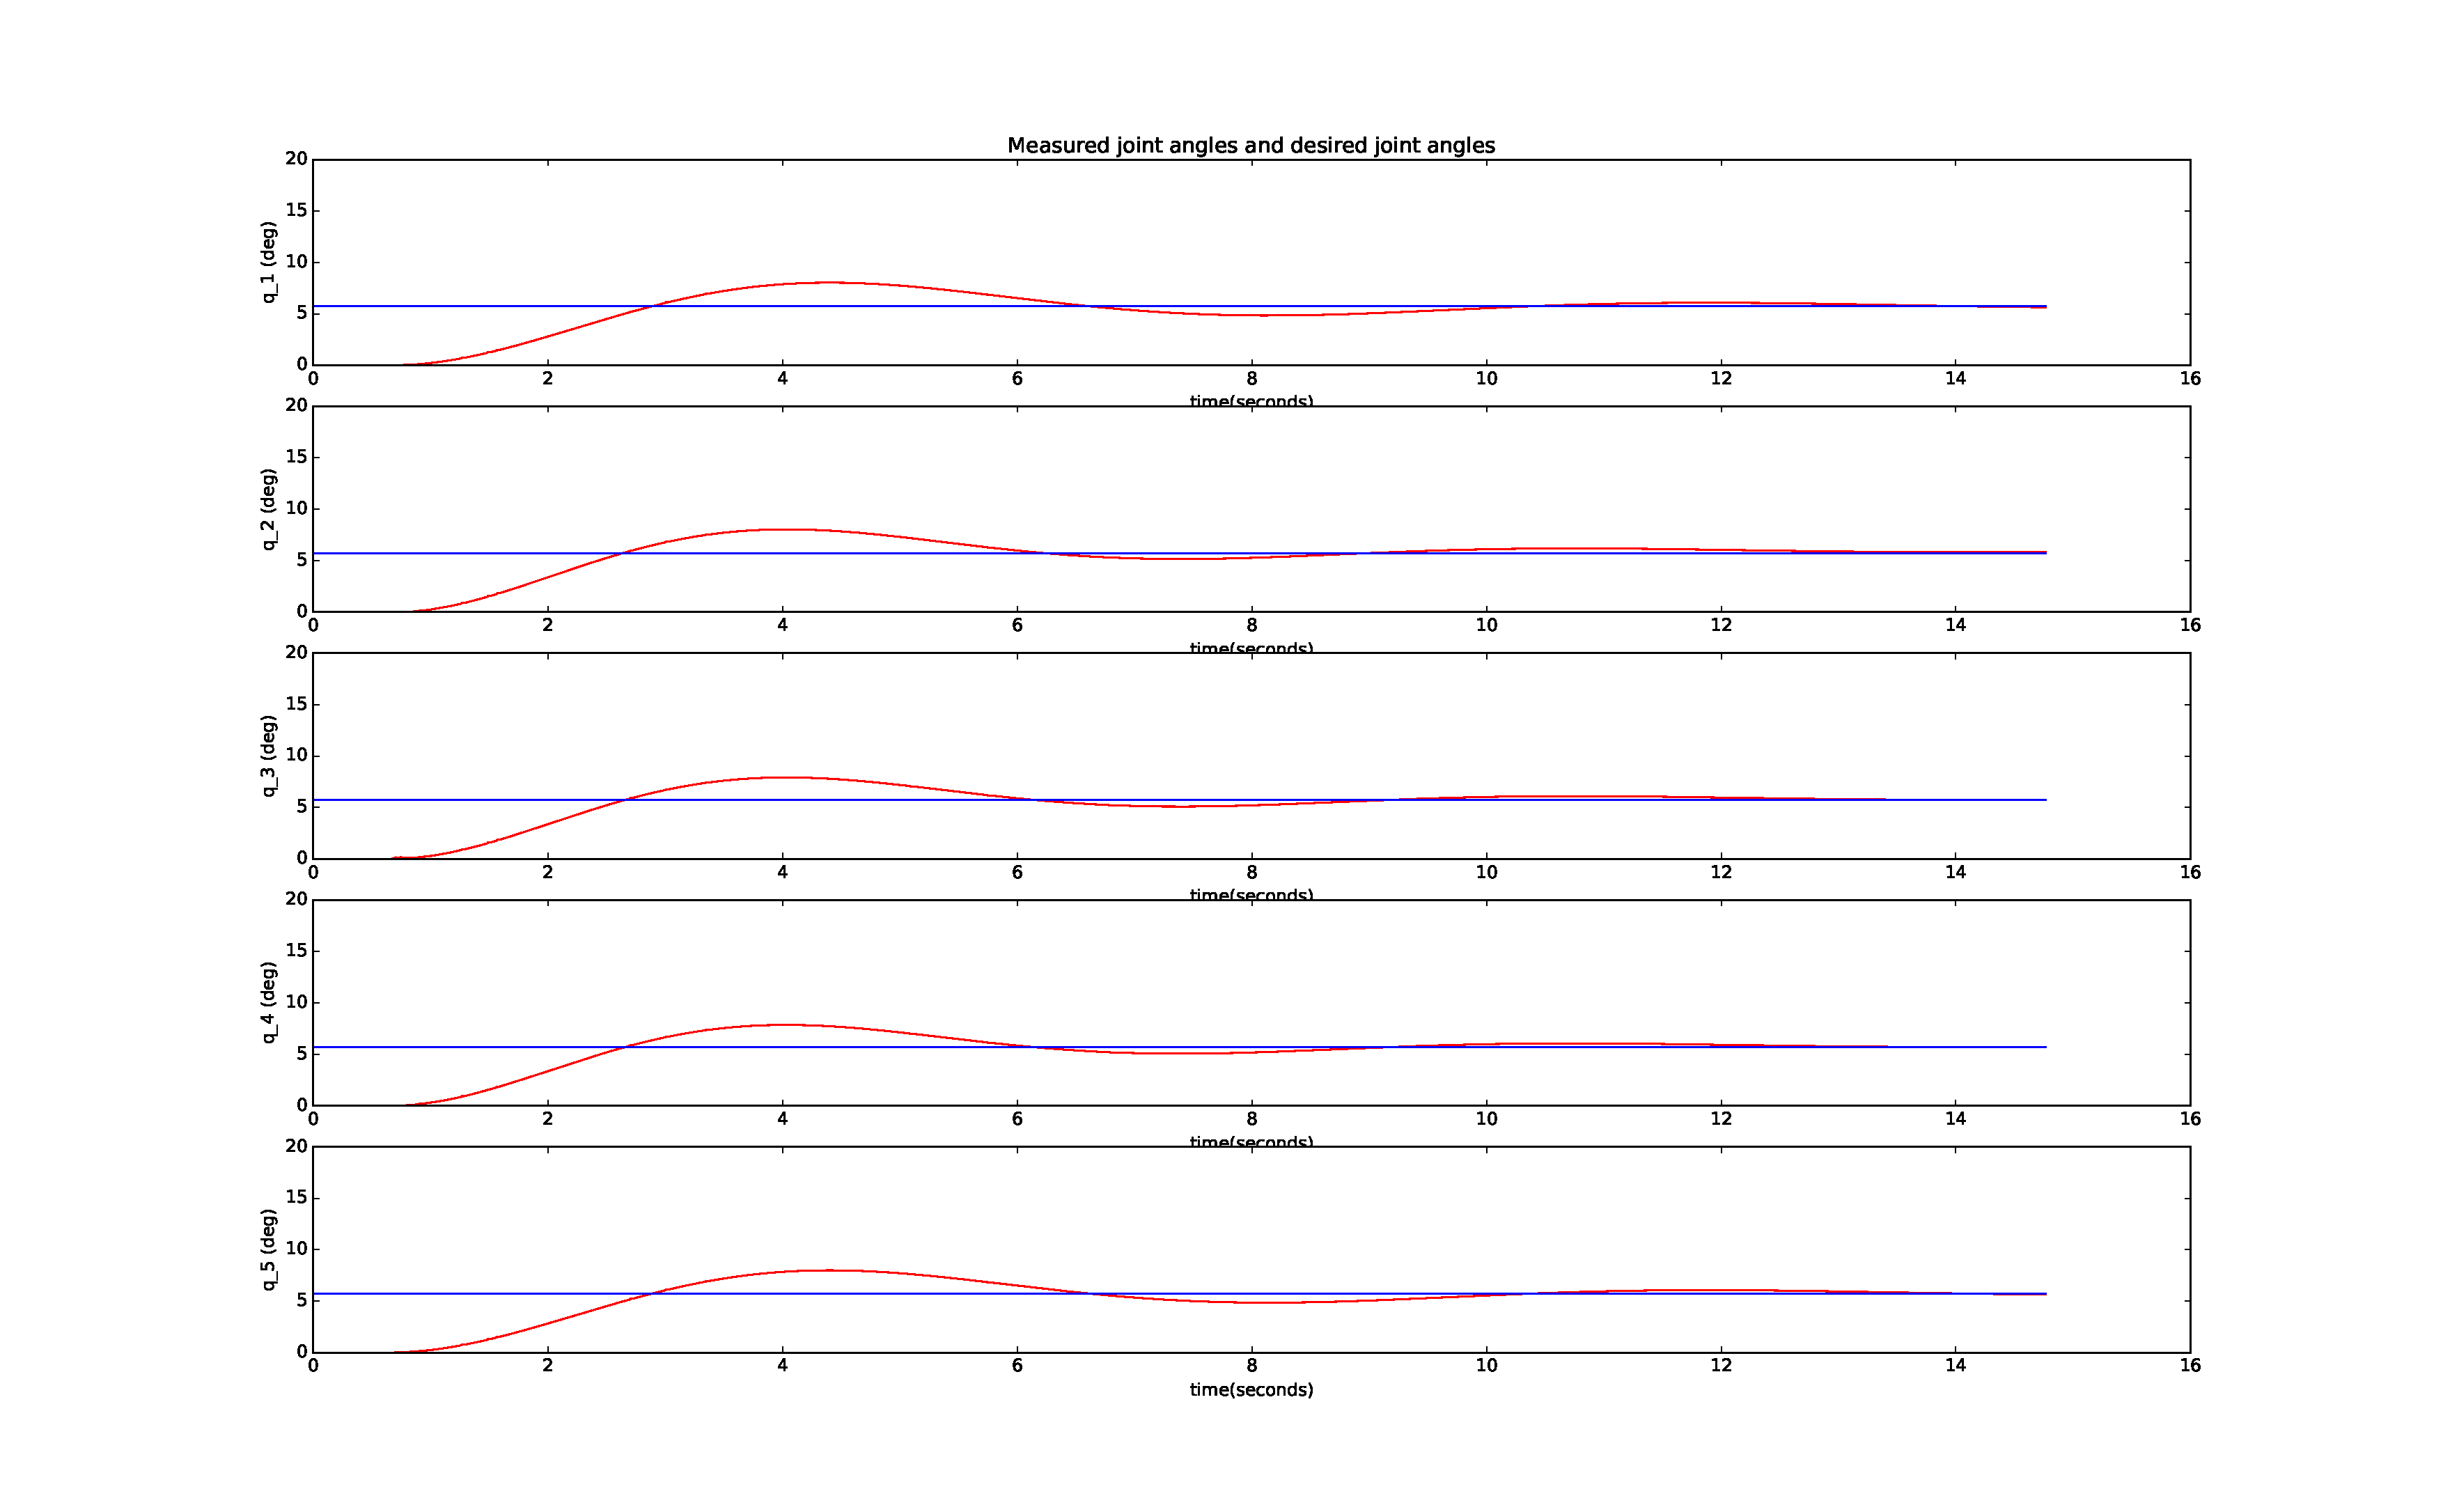
\includegraphics[width=.9\textwidth]{img/joingangKp2.eps}
  \caption{}
  \label{fig:testkp2}
\end{figure}

\subsection*{Spline - interpolation}
The next step now is to make a spline to make more setpoints such that the steps are not so big. This can lead to better behaviour for the robot. 

\subsubsection*{Circle of acceptance}
One problem when calculating the next point is to jump to the next setpoint if all the joints has approached the same step or should it be individual steps such that all the joints settles at different time or all joint settles at the same time. 
